\chapter{风险评估实验和远程入侵模拟测试}
\label{ch5}
\section{实验环境}
本章节首先通过Isograph AttackTree+对其进行安全威胁建模并对其进行风险评估的实例。
其次通过远程入侵渗透测试实现远程获取汽车信息和控制汽车。
\subsection{实验对象}
实验环境:智能网联汽车一台,Windows系统计算机和无线路由器一台。软件环境:手机系统版本为MIUI 10,并安装了手机智能互联APP)。
由于车辆本身就具备了通过车连APP远程控制的功能,因此,在第四章提出的实例威胁建模后,我们对它进行了一个基于模型的仿真实验,结果表明,目前ICV的应用还存在很多安全隐患。

\begin{figure}
    \centering
    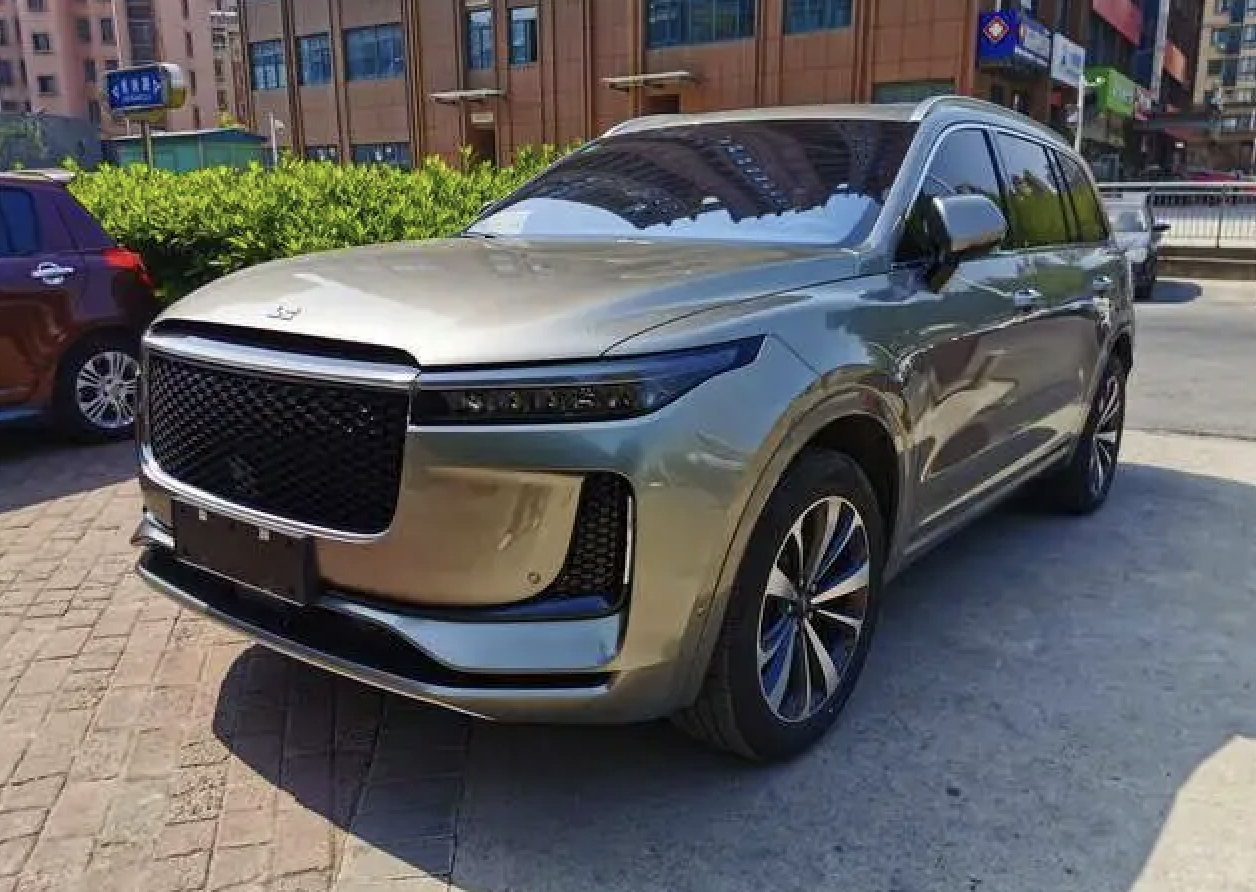
\includegraphics[scale=0.5]{resources/img/i14.png}
    \caption{测试车辆}
  \end{figure}
\subsection{车辆内部架构}
\subsection{实验工具}  

Isograph Attack+ 是著名的安全行业Isograph公司推出的基于攻击树的系统漏洞建模工具。该软件通过建立系统漏洞模型,利用威胁分析和攻击树提高安全性。构建旨在减少成功攻击的措施的图形表示,并使用缓解树。
根据ISO 26262、ISO/SAE 21434、J3061、DO-356和ED-203等标准,该软件可以通过威胁分析和攻击树来确定系统易受攻击的位置,进而提高资产和IT系统的安全性。使用缓解树的图形化表示,我们能够快速构建模型,并且采用AttackTree的高级GUI特性进一步优化模型。此外,我们还可以链接到需求管理工具,如Jama Connect®,以进一步提高产品的安全性和可靠性。该公司产品自上世纪80年代以来一直处于不断的发展过程中,是安全和可靠性专业人士公认的标准。

该软件具有以下优势和特色:

\begin{itemize}
  \item \textbf{可视化潜在的攻击场景:攻击树分析提供了一种以易于理解的图形方式对系统威胁进行建模的方法。如果我们了解系统受到攻击的方式,我们就可以制定对策来防止这些攻击实现其目标。}
  \item \textbf{可以在其中快速构建和分析攻击树模型,并以易于理解的格式呈现结果。AttackTree 还允许用户定义量化攻击成本的指标、发动攻击的操作难度以及可能感兴趣的任何其他相关量化指标。}
  \item \textbf{可以构建缓解树。其功能是用来构建减少攻击带来的影响因素。比如现实生活中公关部门如果通过有利良好的发言可以减缓银行抢劫带来的影响,反之则不然。我们通过构建缓解树模拟现实中这种情况。}    
\end{itemize}
\section{实验过程}
\begin{figure}
  \centering
  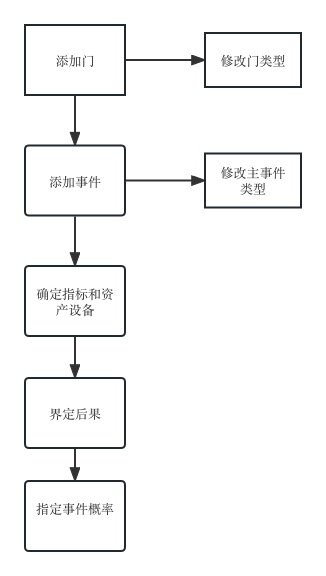
\includegraphics[scale=0.8]{resources/img/c51.png}
  \caption{软件建模流程图}
\end{figure}
我们通过Isograph AttackTree 实现攻击建模,流程如图5.2所示
\subsection{攻击路径分析}
攻击场景选择以恶意攻击IVI系统作为攻击目标,其可能的
攻击类型目前选用了四种:欺骗攻击、篡改攻击、重放攻击、嗅探攻击。
\subsection{构建攻击树}
使用Attack Tree 工具对上述攻击入口进行构建攻击树模型
并编译,根节点定义为恶意攻击IVI系统,叶子节点代表了攻击事件。

\section{实验结果分析}
我们把攻击序列重新评分了一张表,并按照第四章提出的SATT威胁建模风险评估方法,求出了每个攻击序列的发生概率和,再通过Attack Tree+ 编译结果如图5.3所示。
\begin{figure}
  \centering
  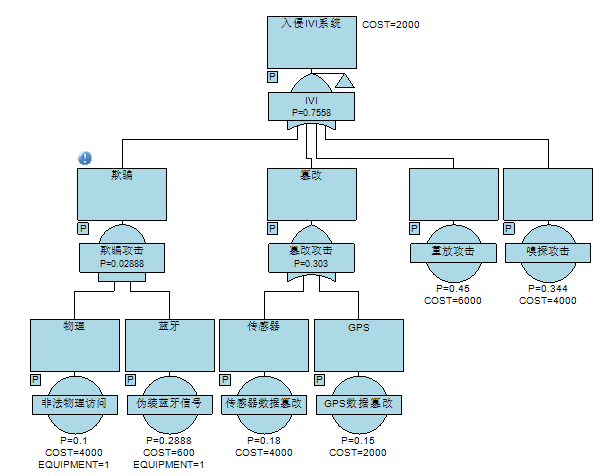
\includegraphics[scale=1]{resources/img/result.pic.jpg}
  \caption{attack tree 仿真实验结果图}
\end{figure}
可以看到综合攻击成本等因素通过GPS篡改信号的攻击路径发生概率最大。由以上仿真实例可知,
SATT安全威胁模型可以为风险评估人员提供更可靠的风险信息,使他们能够更方便地制定下一步的应对策略。

\section{远程渗透及攻击测试}

我们通过几个攻击入口试图对车辆进行远程渗透和攻击测试,
整体的流程如图 5.4所示。大致分为蓝牙信号截取、请求伪造、和逆向工程
几个步骤。我们通过多次可重现实验确定该车存在以下安全漏洞;首先在近距离通信使用蓝牙伪造请求攻击, 具体来说首先分析蓝牙协议配对握手协议,然后找到对应指令操作请求
通过同一局域网PC进行伪造请求 从而达到远程控制智能网联汽车的目的;在逆
向工程部分,下载反编译工具,如apktool、dex2jar和JD-GUI等。接着获取APK文件。然后使用apktool解压APK文件,得到smali代码和资源文件。使用dex2jar将DEX文件转换成JAR文件,得到Java代码。使用JD-GUI查看Java代码,并进行修改。最后从中验证并找到对应关键代码。
\begin{figure}
  \centering
  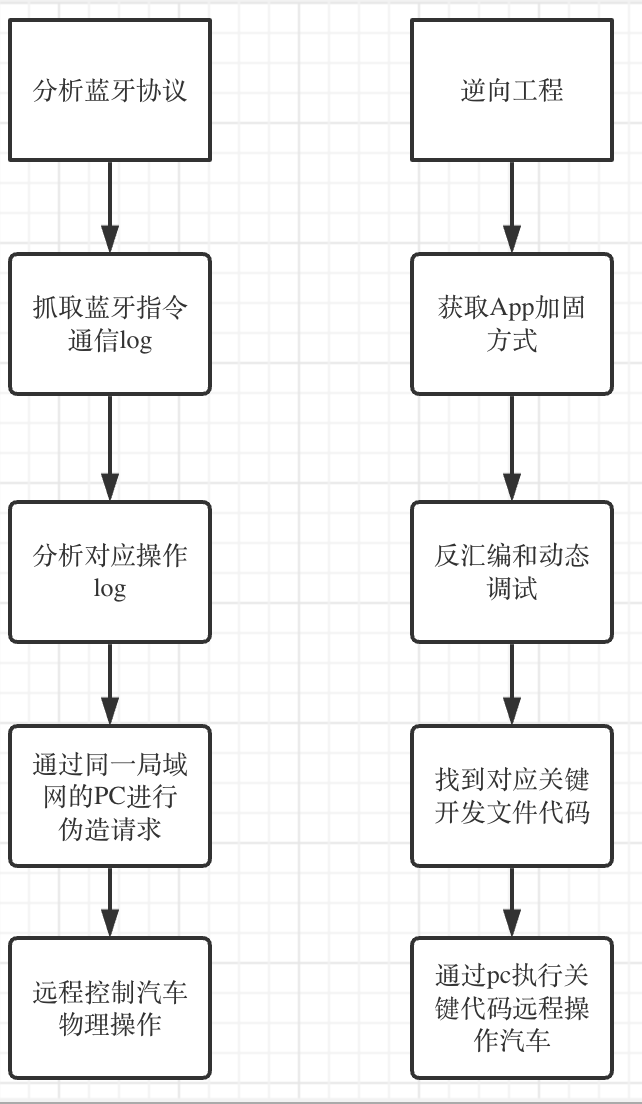
\includegraphics[scale=0.5]{resources/img/i23.png}
  \caption{漏洞挖掘和攻击步骤图}
\end{figure}
\newline
\subsection {蓝牙近距离通信漏洞利用}
Bluetooth是一种近距离数据交换的通信方式,攻击者可以利用其攻击智能网联汽车。
利用 Bluetooth技术,攻击者可以对汽车上的IVI信息系统进行恶意编程,从而入侵汽车网络。文献\cite{antian}
利用蓝牙漏洞,攻击者可利用一系列与蓝牙相关的安全漏洞,在一定场景下可实现对具有蓝牙功能的远端设备的控制,进而窃取受害者数据。
如利用蓝牙技术可实现连接手机或其他设备,实现对汽车的解锁、启动等功能,
蓝牙钥匙功能的优点在于便携、安全,避免了传统车钥匙的遗失和被盗风险,同时增强了用户的驾驶体验。
\subsubsection{蓝牙通信前置知识}
在将手机与系统正确连接后,蓝牙允许的功能是通过车辆通过仪表板、控制屏幕、方向盘按钮或语音命令完全无线访问手机的呼叫功能。
蓝牙既是无线标准又是通信协议,使用一套既定的硬件和编码在您的汽车和手机之间来回发送呼叫和数据,安全可靠。
使用 2.4 GHz 至 2.485 Ghz 的频率,蓝牙硬件以相对较低的功率进行广播——提供仅几英尺(或在某些情况下可达 100 米)的范围,同时节省手机的电池电量并减少暴露于潜在有害辐射.
为了将手机(如 iPhone 或 Android 智能手机)与车辆的蓝牙系统一起使用,需要与系统“配对”——本质上是批准双向通信和远程操作。设备配对一次后,系统会记住它,每次都自动连接。

如图5.5 当两个设备使用传统蓝牙进行连接时,其中一个设备作为搜索设备,另一个设备作为被搜索设备。在连接过程中,搜索设备会以高速进行跳频,而被搜索设备会以低速进行跳频,以确保两个设备能同时跳到同一频段(79个频段中的一个)。然后,搜索设备和被搜索设备会建立连接,并按照跳频图进行连接信道的有规律变化。建立连接后,双方可以根据已建立的逻辑和基于BR/EDR控制器的L2CAP,协商使用可用的AMP控制器,以提高蓝牙传输效率。
对于低功耗蓝牙,同样有两个设备,一个作为广告发送方(Adversting),发送广播包(advertising packets),另一个设备作为扫描器(Scanner),接收广播包。当扫描器接收到"connectable advertising packet"时,会回应"connection request",建立起点对点链接(Initiators)。建立连接后,发起连接的一方成为Master,接受连接的一方成为Slave。频道的选择则取决于Master生成的Hopping Pattern。
\begin{figure}
    \centering
    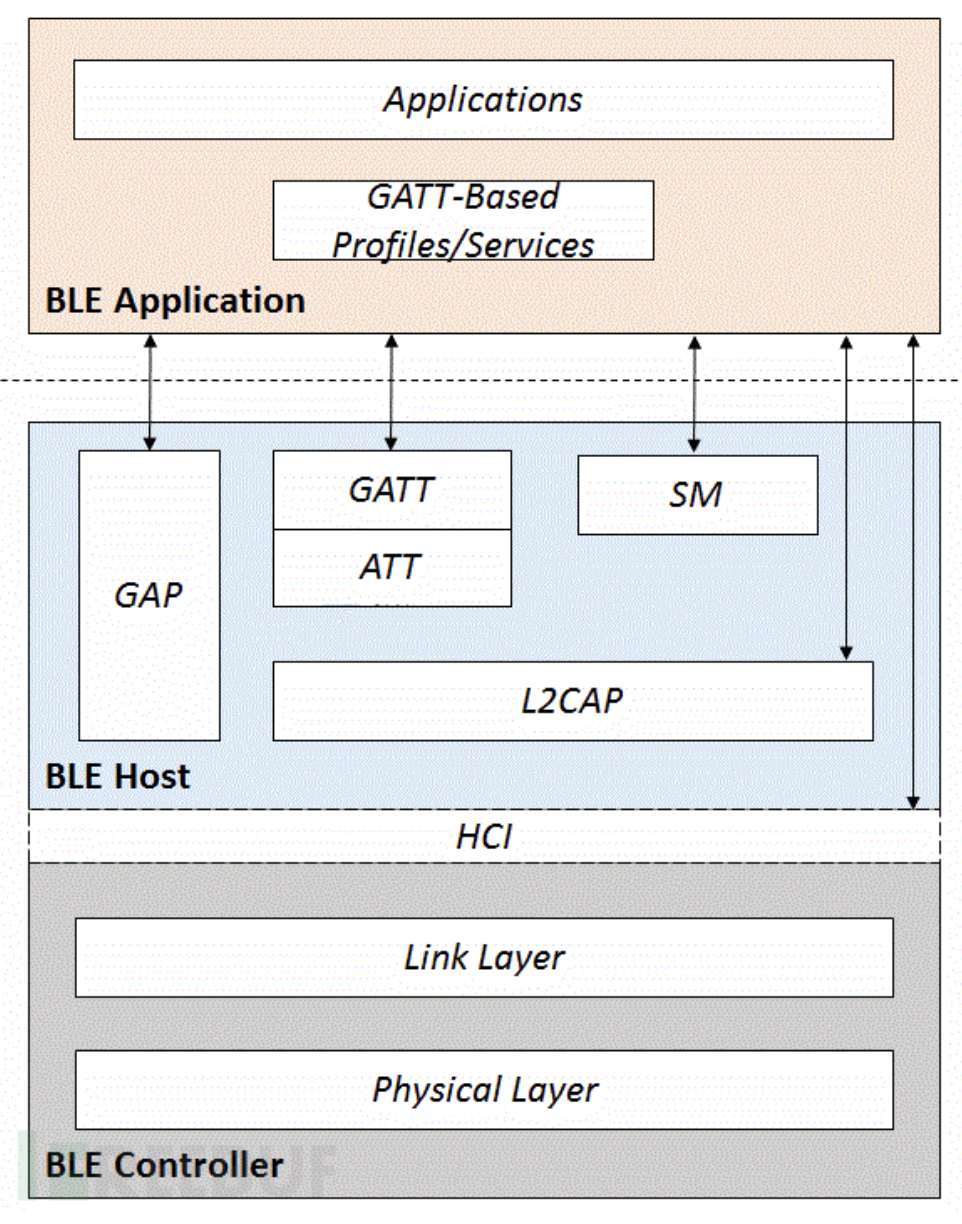
\includegraphics[scale=0.5]{resources/img/i15.png}
    \caption{蓝牙握手协议示意图}
  \end{figure}

\subsubsection{蓝牙协议配对流程}
\begin{itemize}
    \item 配对发起者(Initiator,总是Master)和配对的回应者(Responder,总是Slave)可以交换足够的信息,以决定在阶段2使用哪种配对方法、哪种鉴权方式。
    配对方法:LE legacy pairing 和 LE Secure Connections(新方法优先支持)
    \item 鉴权 如果双方都支持OOB鉴权,则选择该方式(优先级最高)否则,如果双方都支持MITM鉴权,则根据双方的IO Capabilities(并结合具体的配对方法),选择合适的鉴权方式
    \item 获取密钥: 最终生成STK用户建立加密连接,建立加密连接后再自行生成LTKS,通过Transport Specific Key Distribution共享双方生成EDIV和Rand用于索引LTK
\end{itemize}

当我们都配置好了就可以手机汽车app抓包了。运行手机汽车互联app就可以被fiddler所截取到数据包了。
通过检测配对的蓝牙协议中,并未发现使用SMP,所以BLE模块和APP之间并不会进行安全的权鉴, 如图5.6
\subsubsection{通过蓝牙实现伪装请求攻击}
具体攻击思路参考这篇文献\cite{von2021method}:
\begin{itemize}
    \item 让安卓设备抓取到发送的信息
    \item 拿到蓝牙信息进行wine shark 过滤出关键信息
    \item 让电脑设备的linux进行数据读写,达到蓝牙操控的目的
\end{itemize}

(1) 安卓设备首先获取root权限进入文件目录,在设备里进入蓝牙目录,找到bt\_stack.conf蓝牙配置文件,然后在在开发者选项里打开蓝牙HCI信息收集日志
此时若继续蓝牙收发数据可观测到控制台出现了/btsnoop\_hci.log文件,这里有我们所需要的打印信息,如图5.5

(2) 通过adb 命令进行手机的连接,导出我们的.log 文件
\begin{figure}
    \centering
    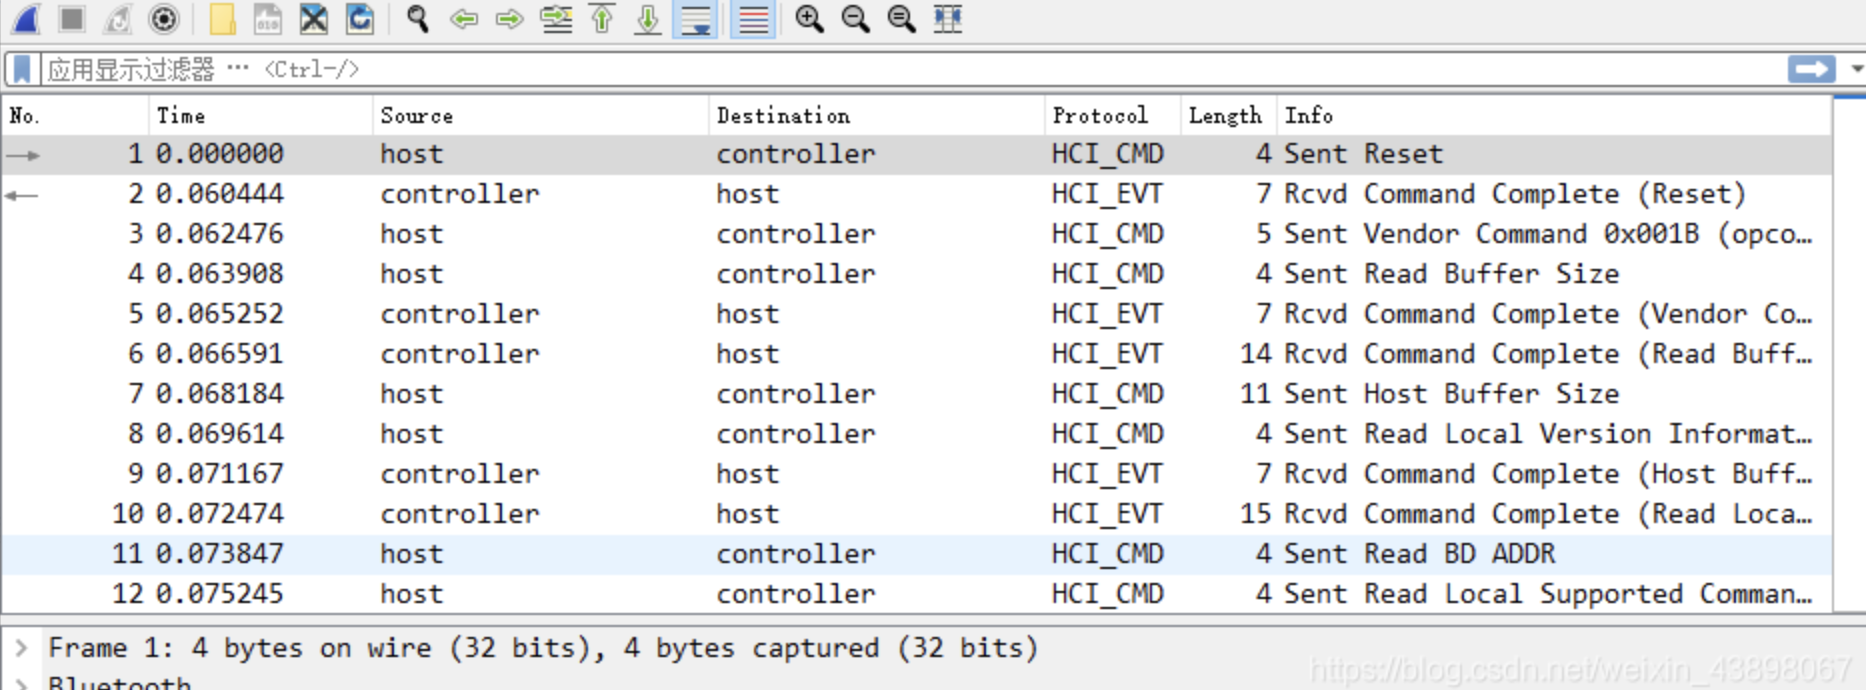
\includegraphics[scale=0.5]{resources/img/i17.png}
    \caption{蓝牙传输数据打印文件图}
  \end{figure}
(3) 通过从手机设置里找到对应的mac地址 我们通过工具过滤出来该设备的蓝牙传输信息。
  
当我们在手机APP下发"开锁"命令时:通过打印工具发现发现:
对应Handle字段为:'0x0019',value是: 313233,
当我们在手机APP下发"解锁"命令时:通过打印工具发现:
对应Handle字段为:'0x004e',value是: 000000。
\begin{figure}
    \centering
    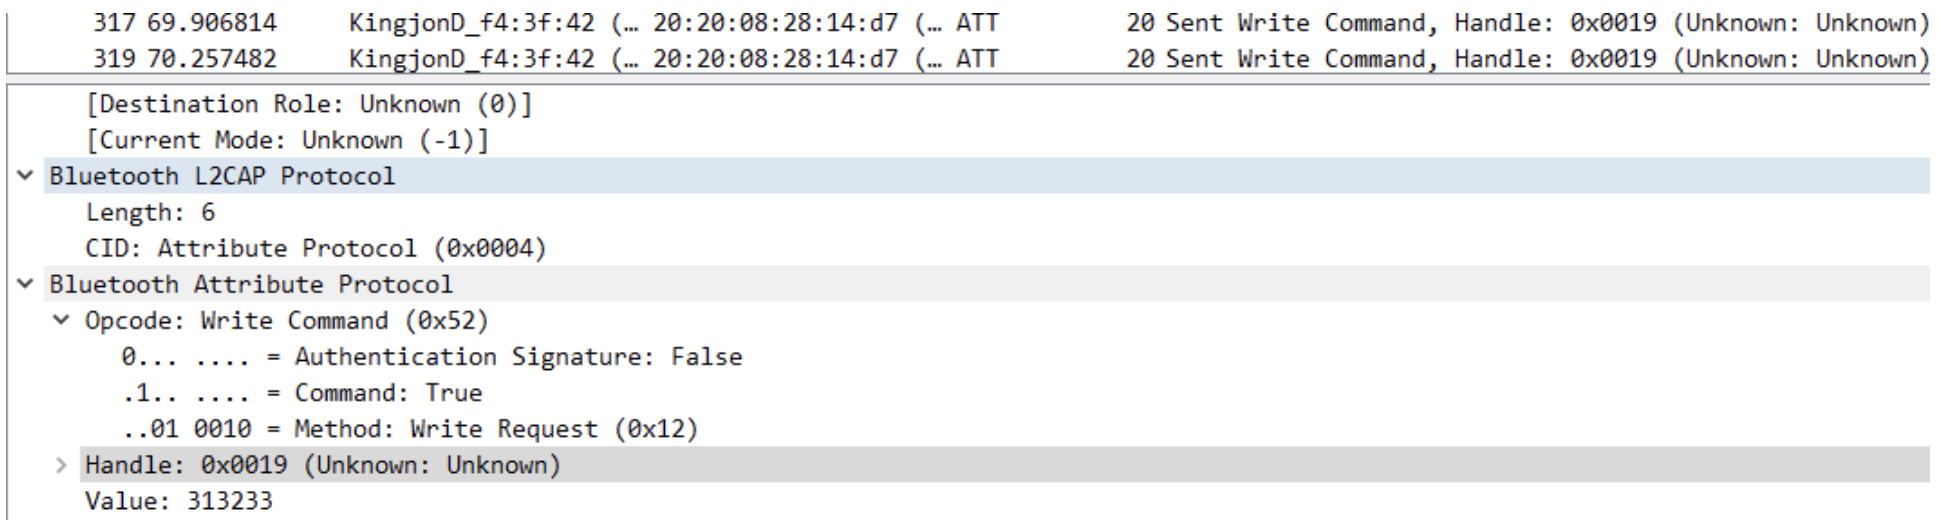
\includegraphics[scale=0.5]{resources/img/i18.png}
    \caption{蓝牙对应操作数据字段图}
  \end{figure}
根据对应字段参数规则,我们可以伪造请求参数\cite{lu2005conditional},
任意的通过pc给配对中的智能网联汽车发送操作指令
从而达到远程恶意控制该智能网联汽车的目的。
此外经过研究和攻击我们还可以通过蓝牙协议对该智能网联汽车进行更多危险的操作。
% \begin{figure}
%     \centering
%     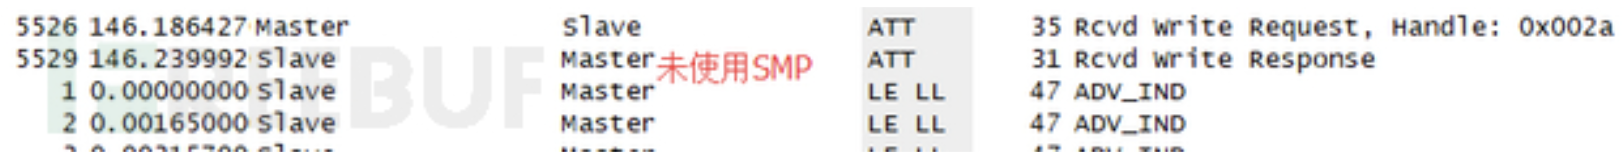
\includegraphics[scale=0.5]{resources/img/i16.png}
%     \caption{蓝牙协议加密图}
%   \end{figure}

\subsection{逆向工程APP和破解请求加密}
我们通过对 App 进行反编译\cite{yang2015automated},可以获取车联网APP源码和对应的接口从而伪造请求获取关键代码。
Android应用程序包(英语:Android application package,APK),APK 是 Android 应用程序的安装包文件的扩展名。这是一种用于 Android 操作系统的应用程序包格式,它包含了应用程序的代码、资源文件和 AndroidManifest.xml 等元数据文件。
APK 文件是开发者将 Android 应用程序编译后生成的文件,也是用户安装应用程序的方式之一。用户可以从各种应用商店、网站或其他来源下载 APK 文件并手动安装应用程序。

\subsubsection{工具准备}
\begin{itemize}
    \item apktool:资源档案,可撷取影像档案及版式档案,供使用者浏览。        
    \item dex2jar:将APK反编译成Java源码(classes.dex转化成jar文件)。
    \item 查看APK中classes.dex转化成出的jar文件,即源码文件 下载apktool、dex2jar、jd-gui,完成后将三个文件放在同一文件中,并解压dex2jar、jd-gui压缩包,这一步是为了方便进行反编译。
\end{itemize}

\subsubsection{执行APK反编译}

\begin{figure}
    \centering
    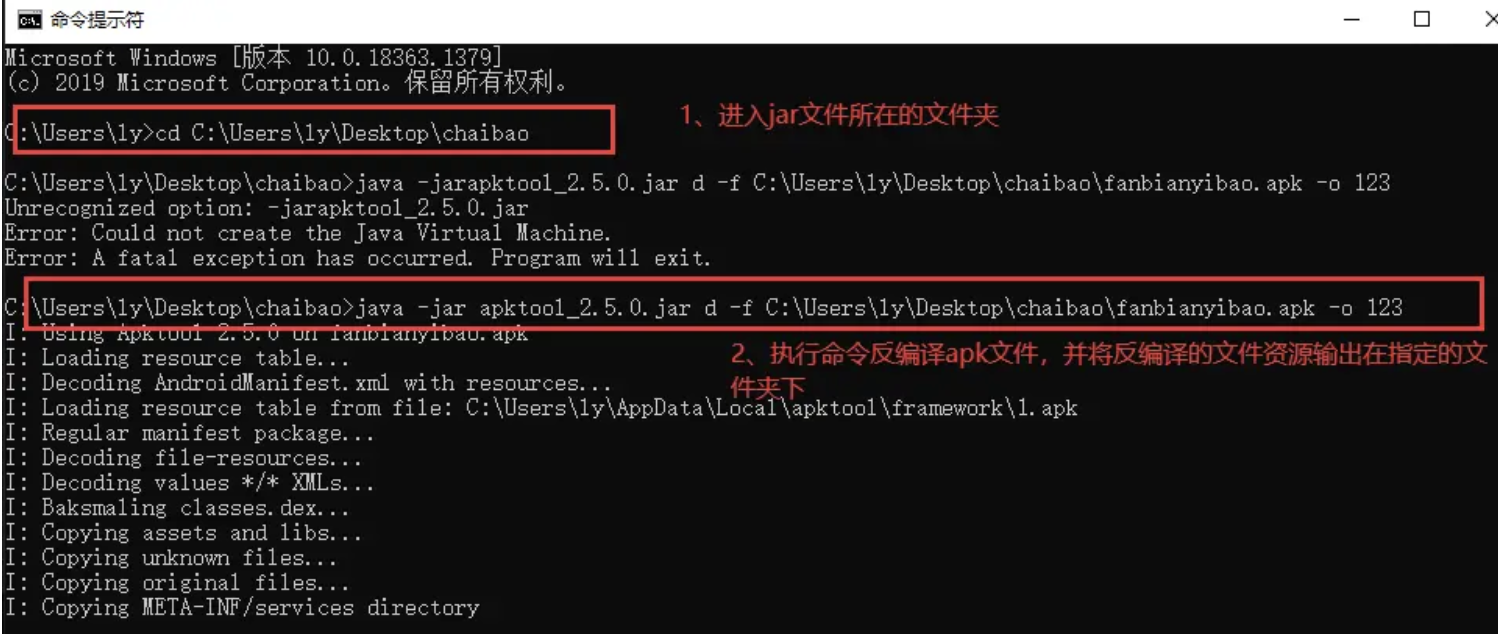
\includegraphics[scale=0.5]{resources/img/i19.png}
    \caption{反编译命令执行行图}
  \end{figure}

  获取反编译成功后文件:打开对应的文件夹可以看到反编译后生成的文件,在这些生成的文件和文件夹当中,
  我们关心的是res文件夹中和AndroidManifest.xml文件,打开res文件夹,里面存放了我们所关心的xml文件,如图5.8所示:
  \begin{figure}
    \centering
    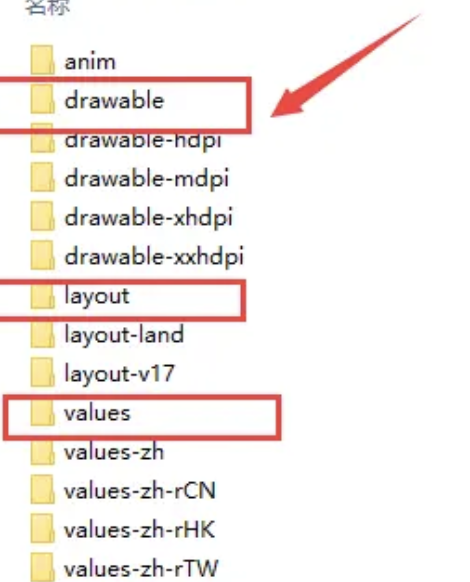
\includegraphics[scale=0.5]{resources/img/i20.png}
    \caption{apk开发文件列表图}
  \end{figure}
  图中展示了APK文件反编译后的资源文件,下面对这些文件做一个简单的介绍:
  \begin{itemize}
    \item META-INF:保存APP的签名信息。
    \item AndroidManifest.xml:Android清单文件,向Android系统提供应用的必要信息。
    \item classes.dex:文件包含了应用程序中所有的Dalvik可执行代码,包括应用程序的所有类、方法、字段以及其他的Java。
    \item assets:存放一些资源文件字体,声音等。
    \item lib:存放第三方库。
    \item original:存放未经过反编译的等AndroidManifest.xml文件。
    \item res:存放资源文件,例如图片、颜色、字符等。
    \item smali:存放Java编译成的smali代码,smali相当于Android虚拟机上运行的语言。
\end{itemize}
\subsubsection{解析加固APK}
APK 加固即通过消除漏洞和增加安全层来“强化”或保护应用程序免受入侵。
加壳过程如图5.10所示,在图中简单的描述了加固的原理,我们自己通过壳程序去加固源APK文件,然后合并两个APK文件。把可程序的DEX文件替换成合并后的DEX文件,此时壳程序可正常运行。这里解释下dex文件的作用:在 Android 应用程序中,.dex 文件是 Dalvik 虚拟机所需的可执行文件。.dex 文件包含了应用程序的所有 Java 代码和相关资源,这些代码在应用程序运行时被 Dalvik 虚拟机执行。
在 Android 应用程序的构建过程中,源代码会被编译成 Java 字节码文件(.class 文件),然后通过 Dalvik 工具链将其转换为 .dex 文件。这是因为 Dalvik 虚拟机采用了一种基于寄存器而非基于堆栈的指令集,因此需要对字节码进行特殊处理。
Android 应用程序的 .dex 文件通常位于 APK 包中的 /classes.dex 文件中。在应用程序启动时,Dalvik 虚拟机会将 /classes.dex 文件加载到内存中,并在运行时解释执行其中的代码。
\subsubsection{脱壳加固APK}
脱壳是把加在软件上的保护程序Dex去掉 直接能看到对应的源码。
跟java类似,安卓的class都是由Classloader的loadClass方法加载的。跟java不同的是,每一个class对象都会有对应的dex对象属性跟相应的dex文件关联起来。利用xposed,将loadClass方法劫持住,每当loadClass方法调用完成后,用xposed执行后置方法。获取方法加载的class对象,然后调用getDex方法。
拿到对应的dex文件引用,最后将dex文件序列成byte数据,写到自定义保存文件里面去。就能拿到脱壳后的dex文件。
我们通过"反射大师"这款软件来进行脱壳处理,其需要在 Xposed 环境中使用,支持市面上大多数加密壳。
\begin{itemize}
  \item 手机或模拟器安装xposed环境
  \item 安装反射大师,xposed内部勾选反射大师模块,重启模拟器。
  \item 打开目标app进入到主界面。
  \item 选择当前ACTIVITY长按写出Dex约两秒后释放,然后点击确定。dex文件可以直接拉到jadx查看源码
\end{itemize}

\begin{figure}
  \centering
  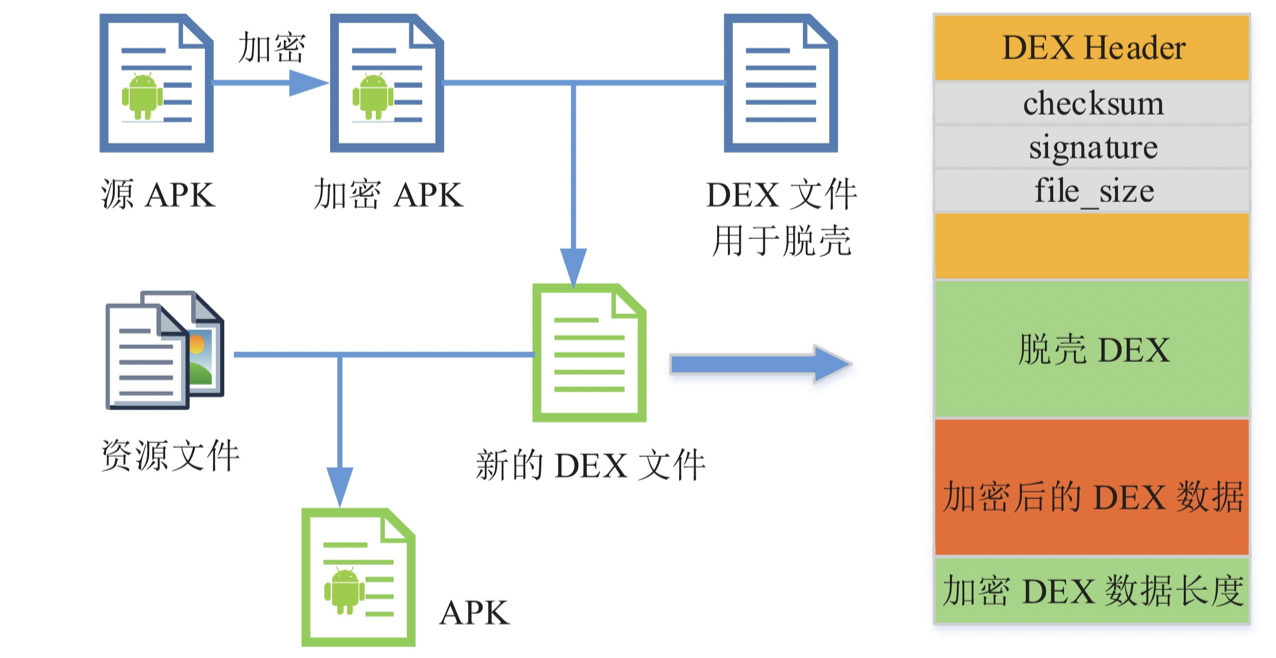
\includegraphics[scale=0.5]{resources/img/i24.png}
  \caption{目标APK加固分析}
\end{figure}

\subsubsection{分析关键操作代码}
\begin{lstlisting}[language=Java,title={获取汽车初始化地理位置代码}]
  private void initLocationStyle() {
    BitmapDescriptor descriptor = BitmapDescriptorFactory.fromResource(R.drawable.main_location_icon);
    MyLocationStyle myLocationStyle = new MyLocationStyle();
    myLocationStyle.myLocationIcon(descriptor);
    myLocationStyle.interval(2000); 
    myLocationStyle.myLocationType(MyLocationStyle.LOCATION_TYPE_FOLLOW);
    myLocationStyle.myLocationType(MyLocationStyle.LOCATION_TYPE_LOCATE);
    myLocationStyle.strokeColor(getResources().getColor(R.color.colorPrimary));
    myLocationStyle.radiusFillColor(getResources().getColor(R.color.colorPrimary_50));
    mMapView.getMap().setMyLocationStyle(myLocationStyle);
    mMapView.getMap().getUiSettings().setMyLocationButtonEnabled(true);
    mMapView.getMap().setMyLocationEnabled(true);
}
  \end{lstlisting}
根据上述代码块只是分析过程中一个关键的部分代码截图,
从图中可看出该初始化了汽车的地理位置以及该文件一系列关于获取地理位置的方法函数,
我们可以通过调用对应方法获取汽车位置信息。
\begin{lstlisting}[language=Java,title={代码块2: 获取汽车经纬度地理位置}]
  public class GeoLocation {
    // 高德秘钥
    private static final String APP_CODE_GAODE = "44aa4b2a7772504960b691cfb9802";

    public static String GetLocationByAddress(String address, String city) {
        log.info("地理编码:address=" + address + ",currentCity=" + city);
        try {
            HashMap<String, Object> parameters = new HashMap<>(3);
            parameters.put("address", address);
            parameters.put("city", city);
            parameters.put("key", APP_CODE_GAODE);

            // 高德获取地理信息
            String response = HttpUtil.get("https://restapi.amap.com/v3/geocode/geo", parameters);
            JSONObject responseJson = JSONUtil.parseObj(response);
            String status = responseJson.get("status").toString();
            if (!"1".equals(status)) {
                log.error("列表信息获取失败,关键字:" + address + "城市:" + city);
                return null;
            }
        JSONArray geocodes = responseJson.getJSONArray("geocodes");
        return JSONUtil.parseObj(geocodes.get(0)).get("location").toString();
        } catch (Exception ex) {
            log.error("调用接口失败!" + ex.getMessage());
            return null;
        }
    }

    public static String GetAddressByLocation(String location) {
        log.info("逆地理编码:location=" + location);
        try {
            HashMap<String, Object> parameters = new HashMap(16);
            parameters.put("location", location);
            parameters.put("key", APP_CODE_GAODE);
            // 高德获取地理信息
            String response = HttpUtil.get("https://restapi.amap.com/v3/geocode/regeo", parameters);
            JSONObject responseJson = JSONUtil.parseObj(response);
            String status = responseJson.get("status").toString();
            if (!"1".equals(status)) {
                log.error("列表信息获取失败,经纬度:" + location);
                return null;
            }
            JSONObject regeocode = responseJson.getJSONObject("regeocode");
            return regeocode.get("formatted_address").toString();
        } catch (Exception ex) {
            log.error("调用接口失败!" + ex.getMessage());
            return null;
        }
    }

}
  \end{lstlisting}
\subsubsection{编写远程控制脚本}
车辆位置跟踪并实现控制车辆运行轨迹。汽车上的导航系统主要依赖 GPS,
如果天气恶劣,还可以利用内置 SIM卡的无线网络基站进行辅助定位。
汽车还配备了 SIM卡和导航地图,可以帮助司机在最短的时间里,找到正确的路线。如果有了网络,就可以连接到云端,
通过在该路段上行驶的车辆的数目来判定前面的道路是否拥堵。根据代码分析,这辆车可以连接到高德地图的 API。这个 ICV的位置经纬度判断是
GPS来确认,最终把数据存储到 TSP云端数据存储中。

我们通过上节逆向工程APK文件编写了定位追踪代码,进行越权
操作 包括:定位追踪、敏感信息获取,以及调用
的 API 的密钥。经纬度可以从 TSP云端数据中通过接口得到,也可以通过调用高德地图 API 获取车辆实时定位。
最后我们通过pc电脑执行代码远程获取了对应车辆的位置信息和其他身份等更敏感信息。如代码块2所示

\subsection{流量抓包和远程登录}
在本节我们通过搭建无线局域网实现APP发送HTTP指令抓包分析, 从而伪造请求参数达到远程向智能网联汽车发出指令的目的。
Cookie是一种存储在客户端的文本文件,用于跟踪和记录用户的会话信息,例如登录信息、购物车内容等。Cookie的工作原理是在客户端(例如浏览器)和服务器之间建立一个状态管理机制,使得服务器可以在多次HTTP请求中识别同一用户的身份和状态。当用户首次访问网站时,服务器会返回一组Cookie,包含一些用户信息和一个唯一的标识符。当用户再次访问该网站时,浏览器会将Cookie发送给服务器,服务器通过解析Cookie来获取用户的会话信息。
session本意是指客户端与服务器的会话状态,由于凭证存储到了服务端,后来也把这些存在服务端的信息称为session。
现在服务器决定自己维护登录状态,仅发给客户端一个key,然后在自己维护一个key-value表,如果请求中有key,并且在表中可以找到对应的value,则视为合法
\begin{figure}
  \centering
  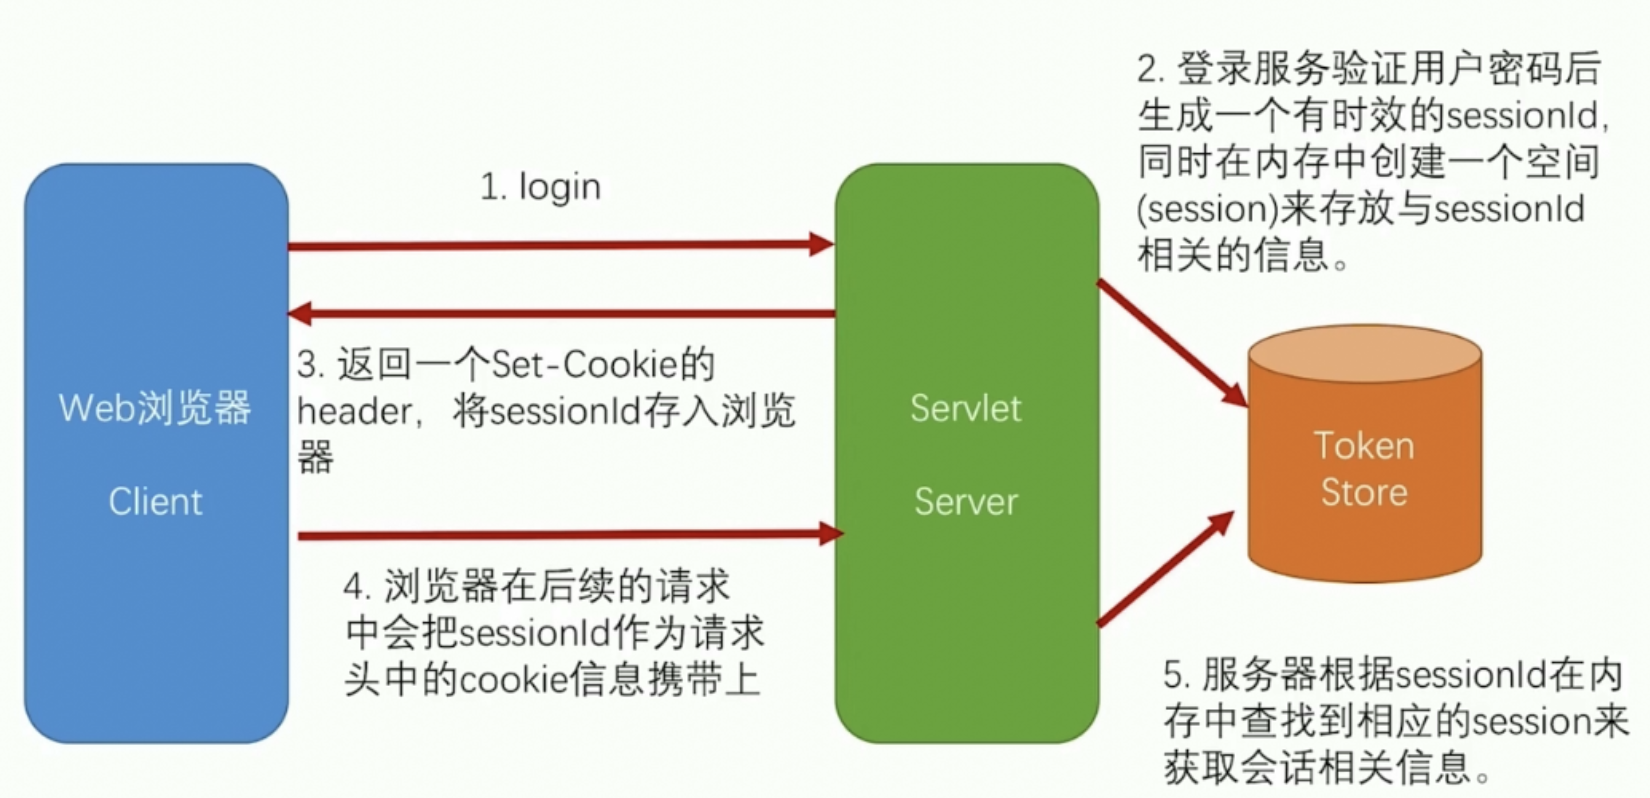
\includegraphics[scale=0.5]{resources/img/i25.png}
  \caption{HTTP请求返回验证Cookie示意图}
\end{figure} 
图5.11为HTTP请求返回验证Cookie流程。
所以,当我们获得另一个客户机的 cookie时,我们可以冒充攻击。
我们先用抓包工具开始抓包HTTP请求,然后查看cookie。
接着在抓包工具复制对应的HTTP请求头数据携带该cookie在程序中发送HTTP请求,
就能让程序伪装APP通过改变参数发出特定的请求操作。
\newline
对数据的抓包流进行分析。
这里我们采用Fiddler\cite{crane2015fiddler}这款软件来进行数据抓取, Fiddler不仅可以抓web页面的HTTP/HTTPS的数据报文, 也可以抓取我们手机移动端的数据报文。
在攻击目标与服务器之间中介,截取并获取用户收发到服务器的敏感信息。
具体步骤如下:
\begin{itemize}
    \item 将手机设置为使用 Fiddler 作为代理服务器,并且确保手机和计算机在同一个网络中。
    \item 配置手机App代理:将手机App代理设置为 Fiddler 的代理,以便所有的网络流量都通过 Fiddler 进行捕获和分析。
    \item 查看抓包结果:在 Fiddler 工具栏上,点击“Inspectors”选项卡,可以查看捕获到的请求和响应。在“Inspectors”选项卡下,可以查看不同的视图,如“Raw”、“Headers”、“JSON”等。
    \item 分析抓包结果:通过分析请求和响应,可以了解每个请求的内容、响应时间、状态码等信息,从而识别出潜在的问题或性能瓶颈。
\end{itemize}

在设置好了Fiddler之后,我们通过车联网APP进行了查看车辆信息(车辆四门开关状态、行驶里程、剩余流量、续航里程、发动机状态)的操作与此同时APP发起了HTTP请求,通过Fiddler我们
成功了侦测到了该请求以及返回数据。如图5.12所示:
\begin{figure}
  \centering
  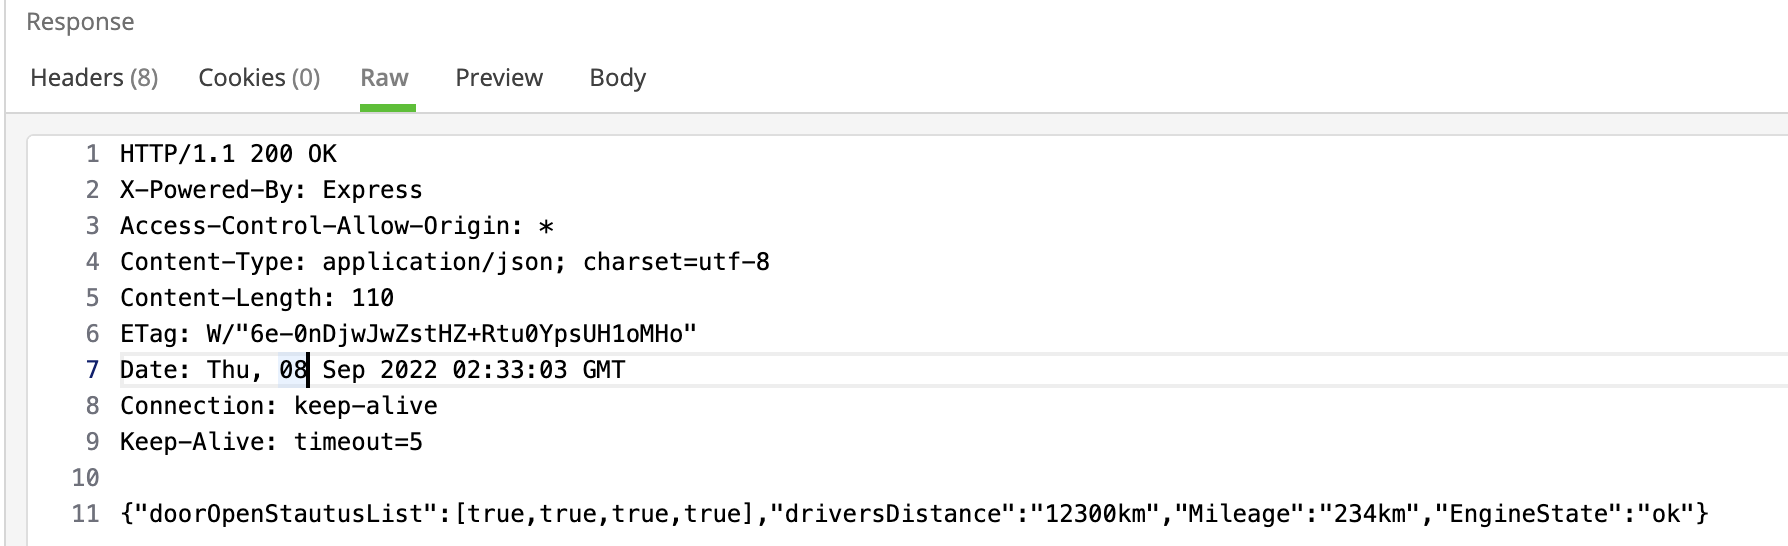
\includegraphics[scale=0.5]{resources/img/i26.png}
  \caption{Fiddler抓取HTTP请求车辆状态信息接口图}
\end{figure}
我们发现手机APP有控制车门开关功能,因此我们通过手机APP点击关门,此时Fiddler也同样侦测到了请求
如法炮制我们利用Fiddler中的Composer功能自定义服务请求发送到服务器,
可以手动创建一个新的请求,也可以在会话表中,拖拽一个现有的请求并进行修改;
因此Composer可以篡改Cookie中的数据。也就是说,Inspectors篡改的是我们输入的数据,这里类似Web安全中CSRF请求攻击\cite{blatz2007csrf},
主要操作步骤如下:
\begin{itemize}
  \item 首先定位到那条开车门请求记录,然后用鼠标将该条请求记录的位置拖拽到Composer中接口。Composer会自动读取到该条请求的所有数据。
  \item 篡改数据。直接在Composer中的Request Body或者是请求头信息中修改数据
  \item 点击“Execute”按钮执行发送请求。
\end{itemize}
由于"开门"“关门”操作是同一个HTTP请求接口只是参数不同,因此我们可以任意的篡改参数任意实现开关门。
\section{防御措施}
对于上述远程攻击,我们提出了一些解决方案,仅供参考。

(1) \textbf{接口加密关键数据}

IVI系统只对某些重要的数据进行了加密,所有接口都会暴露敏感的消息
息,并且有可能会收到恶意的攻击。所以,要实现车载TSP系统和远程设备之间的安全通讯, TSP必须做到以下几点:
加密更多关键信息,或者尽量降低已加密数据与纯文本的耦合。

(2) \textbf{安全认证和访问控制。} 

TSP一般存在不合理的云身份验证结构,造成用户名泄漏
以及修改口令。黑客可以通过假冒用户的身份进行非法登陆,从而对用户的安全造成极大的威胁。
通过 HTTP(S)来阻止对某个 IP的处理也能避免黑客行为以及提升系统防火墙以及提高对SQL注入的认知都能提升系统的安全性。

(3) \textbf{应用逻辑混淆和安全加固。} 

在应用程序中集成混淆工具如Proguard等,这能极大的增加黑客的破解难度;
将代码的最重要部分保留在 C/C++ 开发代码中,这样即便黑客攻克了开发代码也很难获取我们的关键代码;
使用 MD5、AES等加密算法加密重要的api 密钥等,这样和安全接口的身份凭证相结合能提升接口安全性;

\section{本章小结}
本章首先通过Isogrash AttackTree 这款软件对商用汽车进行了仿真实验,验证了我们提出的安全威胁模型的可行性。
其次,再进行真实的远程渗透攻击的实验。先进行蓝牙近距离通信伪造操作请求 成功的发送伪造请求 解锁了车辆车门;
然后破解解析车联App,从而获取车主个人信息及汽车内部信息和状况;最后我们通过抓包手机互联APP发送的汽车操作HTTP请求获得了登录凭证Token
通过该凭证我们实现了伪造请求远程操控智能网联汽车的入侵行为。
